\section{Projektowanie, testowanie i uruchamianie układu SoC}

\subsection{Konstruowanie układu SoC z użyciem systemu LiteX}

O ile układ SoC można zaprojektować w całości od podstaw, częstą praktyką jest wykorzystywanie gotowych komponentów, często napisanych przez zewnętrznych dostawców, w celu szybszego zaprojektowania układu spełniającego założenia projektowe.

LiteX\cite{https://doi.org/10.48550/arxiv.2005.02506} jest zbiorem narzędzi oraz komponentów, pozwalający na zbudowanie zarówno kompletnego układu SoC, jak i bardziej specjalizowanych systemów w formie syntezowalnej logiki. W tym celu wykorzystuje bibliotekę Migen\cite{migen:2016:Online}, która implementuje język opisu sprzętu w formie obiektów w języku Python\cite{10.5555/1593511}. Dzięki temu możliwe jest opisanie logiki z wykorzystaniem jednego z popularnych języków programowania, co zmniejsza barierę wejścia; oprócz tego można wykorzystać narzędzia z ekosystemu języka Python, dzięki czemu dostępne są między innymi większe możliwości parametryzacji logiki czy systemy do przeprowadzania testów automatycznych. Jednocześnie możliwe jest łączenie logiki napisanej w innych językach, co ułatwia wykorzystywanie komponentów spoza zestawu LiteX.

\begin{figure}[H]
\centering
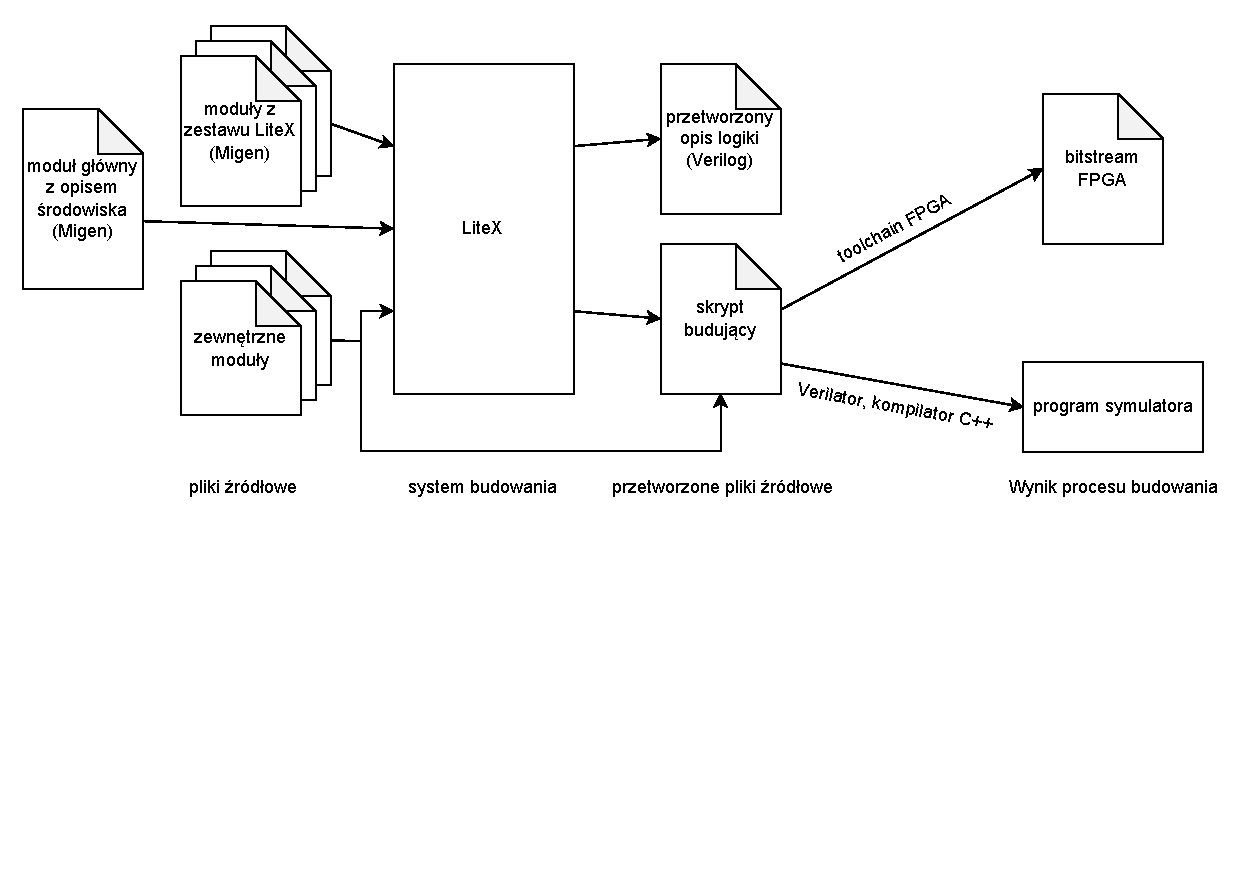
\includegraphics[scale=0.7,trim={0 6cm 0 0.3cm},clip]{tooling/diag-litex.pdf}
\caption{Struktura projektu układu logicznego opartego na systemie LiteX}
\label{fig:litex-project-schem}
\end{figure}

Na rysunku \ref{fig:litex-project-schem} przedstawiona została struktura projektu układu logicznego zbudowanego z wykorzystaniem systemu LiteX. Elementy takie, jak generowanie skryptów budujących układ logiczny czy podstawowe peryferia wejścia/wyjścia są integralną częścią tego systemu, co pozwala użytkownikowi skupić się na tworzeniu samego układu. Główną część układu, definiującą między innymi połączenia między komponentami oraz sygnały wejścia/wyjścia, opisuje się w języku Python z użyciem biblioteki Migen. Opis ten na etapie budowania, łącznie z dodatkowymi modułami wykorzystującymi bibliotekę Migen, jest przetwarzany następnie do formy kodu opisu sprzętu w języku Verilog. Możliwym jest też dodanie komponentów zaimplementowanych w językach Verilog oraz VHDL --- w tym wypadku źródła nie są przetwarzane, tylko są przekazywane bezpośrednio do skryptu budującego. Skrypt budujący, w zależności od opisu platformy docelowej, może zbudować projekt do formy pliku binarnego dla układu FPGA z użyciem dedykowanych narzędzi lub zbudować program symulatora, który można uruchomić na komputerze osobistym.

LiteX został wybrany jako podstawa tego projektu ze względu na dużą popularność tego systemu w otwarto-źródłowych projektach wykorzystujących układy FPGA oraz z powodu doświadczenia autora niniejszej pracy nabytej poprzez wykorzystanie go w swoich poprzednich projektach.

\subsection{Symulowanie układu z użyciem LiteX i Verilator}

LiteX zawiera modularne środowisko symulacji, które pozwala na symulację zaprojektowanego układu na podstawie opisanej w języku Migen logiki oraz parametrów dotyczących środowiska zewnętrznego. Możliwe jest dzięki temu przetestowanie układu oraz przeznaczonego na nie oprogramowania, przykładowo poprzez wykorzystanie wirtualnego interfejsu Ethernet do komunikacji. Ułatwia to usuwanie błędów z projektu układu, jak i oprogramowania, zanim jeszcze układ zostanie zsyntetyzowany do formy bitstreamu dla układu FPGA na potrzeby dalszych testów.

\begin{listing}[H]
\begin{minted}{python}
class SimSoC(TestSoC):
    def __init__(self, local_ip, remote_ip, **kwargs):
        # Inicjalizacja platformy symulatora z podanymi sygnałami
        platform = SimPlatform("SIM", _io)
        sys_clk_freq = int(1e6)
        crg = CRG(platform.request("sys_clk"))
        self.local_ip = local_ip
        self.remote_ip = remote_ip

        # Klasa TestSoC implementuje współdzielone części opisu układu SoC
        TestSoC.__init__(self, platform, sys_clk_freq, crg, uart_name="sim", **kwargs)

        # Dodanie kontrolera Ethernet
        self.submodules.ethphy = LiteEthPHYModel(self.platform.request("eth", 0))
        self.add_etherbone(phy=self.ethphy, ip_address=self.local_ip)

        # Dodanie modułu do debugowania układu
        platform.add_debug(self, reset=0)
\end{minted}
\caption{\label{lst:tooling-litex-sim-soc}Klasa SimSoC opisująca układ w formie przeznaczonej do symulacji}
\end{listing}

W celu uruchomienia naszego systemu w symulatorze układ musi zostać przetworzony do formy kodu programu komputerowego. W tym celu LiteX integruje obsługę programu Verilator\cite{verilator:2016:Online} w celu konwersji układu do kodu komputerowego w formie źródłowej. Ów program łączony jest z dodatkowymi modułami, które łączą naszą logikę z dodatkowymi modułami; pozwalają one na symulację wybranych peryferiów z użyciem zasobów systemu operacyjnego. W przypadku tego projektu będzie to interfejs szeregowy UART dostępny w formie standardowego strumienia wejścia/wyjścia oraz niewykorzystany interfejs Ethernet w formie wirtualnego interfejsu sieciowego w systemie hosta. W ten sposób symulacja układu nie różni się znacząco od wykonywania programu komputerowego, co ułatwia interakcję z programem wykonywanym w wirtualnym środowisku.

\begin{listing}[H]
\begin{minted}{python}
class SimSoC(TestSoC):
    # Funkcja opisująca elementy symulatora, które będą wykorzystywane
    # do generowania sygnału zegarowego oraz interfejsów wejścia-wyjścia
    # dostępnych dla użytkownika
    def get_sim_config(self):
        sim_config = SimConfig()w celu przygotowania modułów do komunikacji z
        sim_config.add_clocker("sys_clk", freq_hz=self.sys_clk_freq)
        cpu = CPUS.get(self.cpu_type)

        # Dodanie interfejsu UART dostępnej z poziomu konsoli symulatora
        sim_config.add_module("serial2console", "serial")

        return sim_config
\end{minted}
\caption{\label{lst:tooling-litex-sim-config}Funkcja opisująca sposób sterowania i komunikacji z testowanym układem z poziomu symulatora}
\end{listing}

W praktyce zbudowanie symulatora układu polega na podmianie wybranych peryferiów na modele, które są częściowo zaimplementowane w formie bibliotek dla symulatora Verilator, oraz na opisaniu wykorzystywanych modułów i sposobu dostępu do nich z poziomu systemu operacyjnego hosta.

\subsection{Testowanie logiki z użyciem biblioteki cocotb}

Standardową praktyką przy testowaniu układów logicznych jest pisanie skryptów testowych (z j. ang. \texttt{testbench}), wykorzystywanych do testowania logiki poprzez sterowanie sygnałami wejściowymi oraz porównywanie stanu sygnałów wyjściowych z oczekiwanymi wzorcami. Owe skrypty są zwykle pisane w tym samym języku, co testowany układ logiczny.

Ze względu na wykorzystywanie języka Python w tej pracy do zaprojektowania układu SoC, dobrym pomysłem jest użycie go również w celu testowania logiki. W tym celu wykorzystana została biblioteka cocotb\cite{cocotb:2022:Online}, która pozwala na testowanie projektów zaimplementowanych w językach Verilog i VHDL z użyciem skryptów napisanych w języku Python. Cocotb współpracuje z zarówno komercyjnymi, jak i otwarto-źródłowymi symulatorami, dzięki czemu można tę bibliotekę wykorzystać w istniejących już środowiskach do projektowania układów logicznych.

\begin{listing}[H]
\begin{minted}{python}
@cocotb.test()
async def test_blink(dut):
    # Przygotowanie testowanego układu oraz generatora sygnału zegarowego
    harness = Harness(dut)
    clk_gen = make_clock(harness.dut, 1)

    # Kroki testu
    # 1. ustawienie poziomu niskiego na sygnale wejściowym `blink`
    await self.dut.blink.value = 0
    # 2. odczekanie dwóch cykli zegarowych
    await ClockCycles(self.dut.clk, 2)
    # 3. ustawienie poziomu wysokiego na sygnale `blink`
    await self.dut.blink.value = 1
    # 4. odczekanie dwóch cykli zegarowych
    await ClockCycles(self.dut.clk, 2)

    # Wyłączenie zegara
    clk_gen.kill()
\end{minted}
\caption{\label{lst:tooling-sampletest}Fragment testu w języku Python realizującego operację odczytu wybranej ilości słów poprzez magistralę Wishbone}
\end{listing}

Jako że ręczne wykonywanie transmisji na magistrali Wishbone oraz interpretowanie ich wyników będzie często powtarzaną operacją, w zamian użyta została biblioteka cocotbext-wishbone\cite{cocotbext-wishbone:2022:Online}, która udostępnia dwa obiekty: monitora oraz sterownika. Sterownik odpowiada stronie inicjującej transfer na magistrali, natomiast monitor obsługuje transfery w ten sam sposób, co peryferium nasłuchujące na magistrali.

\begin{listing}[H]
\begin{minted}{python}

@cocotb.test()
async def test_blink(dut):
    # Inicjalizacja kontrolera Wishbone
    self.wbs = WishboneMaster(dut, "io_wbs", dut.clock,
                          width=32,   # szerokość szyny danych
                          timeout=10) # maksymalna długość czekania na odpowiedź

    # Odczytanie czterech wartości ze określonych adresów
    wbRes = async self.wbs.send_cycle([WBOp(2), WBOp(3), WBOp(0), WBOp(1)])
\end{minted}
\caption{\label{lst:tooling-cocotbext-wishbone-example}Fragment testu w języku Python wykorzystującego bibliotekę cocotbext-wishbone w celu wykonania operacji odczytu na magistrali Wishbone}
\end{listing}

Wspomniana biblioteka cocotbext-wishbone została rozbudowana o przekazywanie i monitorowanie stanu dodatkowych sygnałów, które zostały uprzednio zdefiniowane w specyfikacji, a nie były wykorzystywane przy standardowych transferach. Pozwoliło to na kontrolowanie i monitorowanie stanu magistrali w testowanych układach po dokonaniu w nich zmian opisanych w następnym rozdziale.

\subsection{Wnioski związane z doborem narzędzi}

Dzięki wykorzystaniu komponentów i narzędzi, udostępnionych na wolnych i otwartych licencjach, możliwym jest realizacja kompletnego systemu jednoukładowego oraz jego testowanie niższym nakładem finansowym, niż wykorzystując komercyjne rozwiązania, które z powodu wysokiej ceny mogą być nieosiągalne dla małych firm i hobbystów.
Dodatkową zaletą jest możliwość łatwiejszej wymiany wiedzy oraz wprowadzania do nich modyfikacji, które mogą zostać wykorzystane przez osoby i firmy trzecie.
Z drugiej strony narzędzia komercyjne stosowane przy projektowaniu systemów jednoukładowych potrafią być, z powodu często dłuższej obecności na rynku, lepiej udokumentowane oraz bardziej znane przez osoby je wykorzystujące do projektów tychże systemów.

Mimo dominacji własnościowych rozwiązań możliwość wspólnego rozwoju narzędzi oraz komponentów powoduje, iż otwartoźródłowe rozwiązania będą stawały się coraz popularniejsze, nawet jeśli nie zastąpią na każdym etapie projektowania i produkcji systemów jednoukładowych popularniejszych narzędzi komercyjnych.
